\section{XACML Policy Refactoring Process} \label{sec:approach}
This section describes our approach and gives an insight of the process supporting it. In the first step, we show how performance improvement can be achieved by
reducing the number of access control rules that have to be considered at the evaluation time, through the definition of policy based splitting criteria. 
Secondly, we explain how to select the splitting criterion that preserves the synergy requirement in the access control architecture.
\subsection{Definition of Policy based Splitting Criteria}
Decision engines performing XACML policy evaluation use brute force searching techniques by comparing a given request with all the rules in a policy.
What happens in a request evaluation process is that for a given access control request, some rules are evaluated in the global policy whereas some of those rules are not
 applicable to the request. Starting from this observation, we propose to evaluate only the relevant rules for a given request in the decision making process. 
We propose to split the initial policy into smaller policies based on attribute values combination. For a given system, we transform the policy \normalsize $P$ into 
policies \normalsize $P_{SC_{w}}$ containing less number of rules and conforming to a Splitting Criteria $SC_{w}$. An $SC_{w}$ defines the set of attributes that are considered 
to classify all the rules into subsets having similar one or more attribute values, $w$ denotes the number of attributes that have to be considered conjointly for aggregating 
rules based on specific attribute elements selection. A policy can be split into a set of sub-policies where the rules have the same values of attributes of subject, resource, or 
action. We envision to consider also two attributes like $<Subject, Action>$ or $<Action, Resource>$, in this setting, a policy will be transformed into a set of smaller 
policies where rules in the resulting policies have the same couple of attribute elements. We can go further in our grouping strategy by considering a triplet of attributes
elements: resource, action and subject to split \normalsize $P$. Table I shows all splitting criteria categories according to the attribute elements combination.
\begin{table}[h!]
\centering
\setlength{\extrarowheight}{6 pt}
\begin{tabular}{|>{\small}c|>{\small}c|} 
\hline  \rowcolor{black} 
\bf
\textcolor{white}{Categories}& \bf \textcolor{white}{Splitting Criteria}\\ \hline
$SC_{1}$& {$<Subject>, <Resource>, <Action>$}\\ \hline
$SC_{2}$& {$<Subject,Action>, <Subject,Resource>$}\\&{$<Resource,Action>$}\\  \hline
$SC_{3}$& {$<Subject,Resource,Action>$}\\ \hline
\end{tabular}
\caption{Splitting Criteria}
\label{table1}\end{table}


Once the splitting process is performed, the access control architecture will include one or more (PDPs) that comply with a certain splitting criterion.
We use SUN's XACML implementation \cite{sunxacml} as a decision engine framework that evaluates the policies against requests.
SUN's XACML. During the evaluation process, the SUN decision engine has to check the request against the policy and to determine whether the request should be
permitted or denied. SUN's XACML implementation permits to load the considered policy in a file which is used during the decision making process, once the applicable policy 
is selected from this file, the decision engine fetches the policy to retrieve the applicable rules that are applicable to the request

\begin{figure}[!h]
\begin{center}
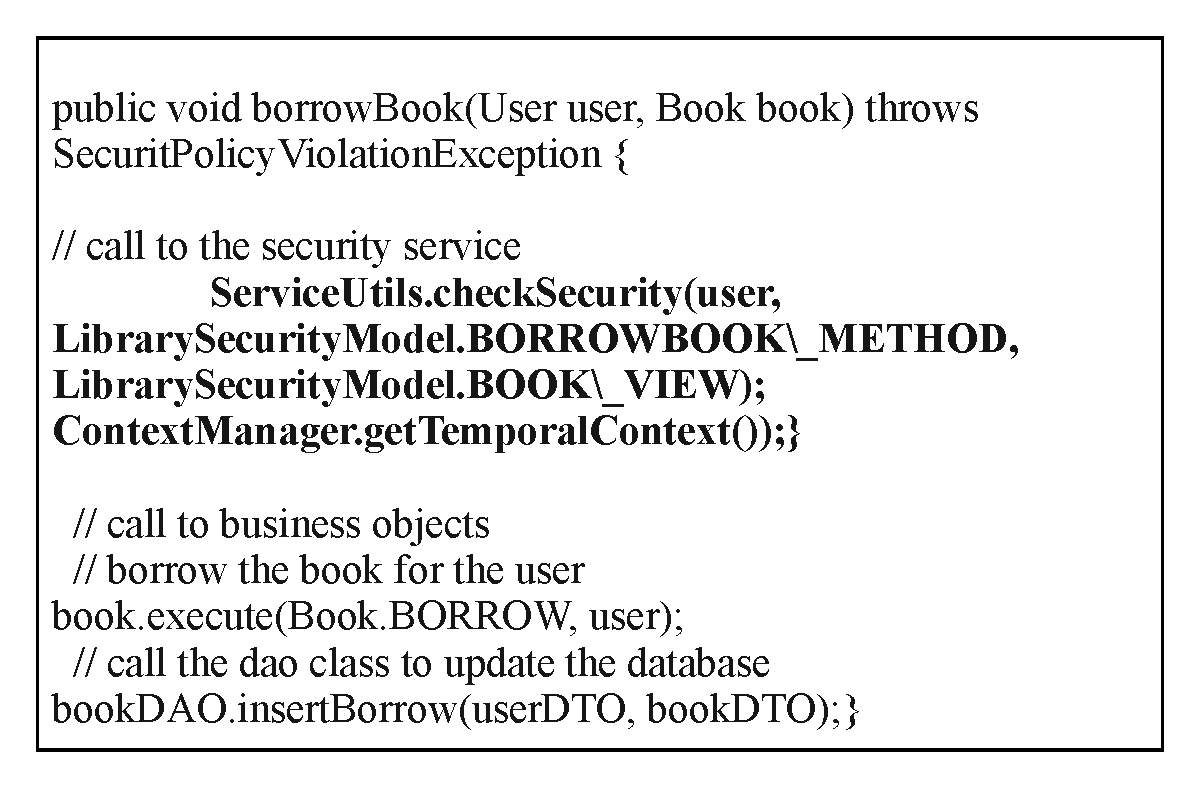
\includegraphics[width=7.5cm, height=4cm]{PEPExample}
\caption{PEP deployment Example}
\label{PEP deployment Example}
\end{center}
\end{figure}
Figure \ref{requestevaluation} compares two evaluation scenarios that takes into account an original policy with an evaluation process that considers resulting policies from he splitting process. 
The first scenario shows how the single policy is selected from the configuration file and how the rules are processed to retrieve the decision, the second scenario shows how the applicable 
policy is selected from the configuration file. Sun's XACML enbales to select the applicable policy, by verifying the matching between the request's attributes and and the policy set attributes. 
After the selection of the applicable policy, all its rules which are considered relevant for the decision making are evaluated.

\begin{figure}[!h]
\begin{center}
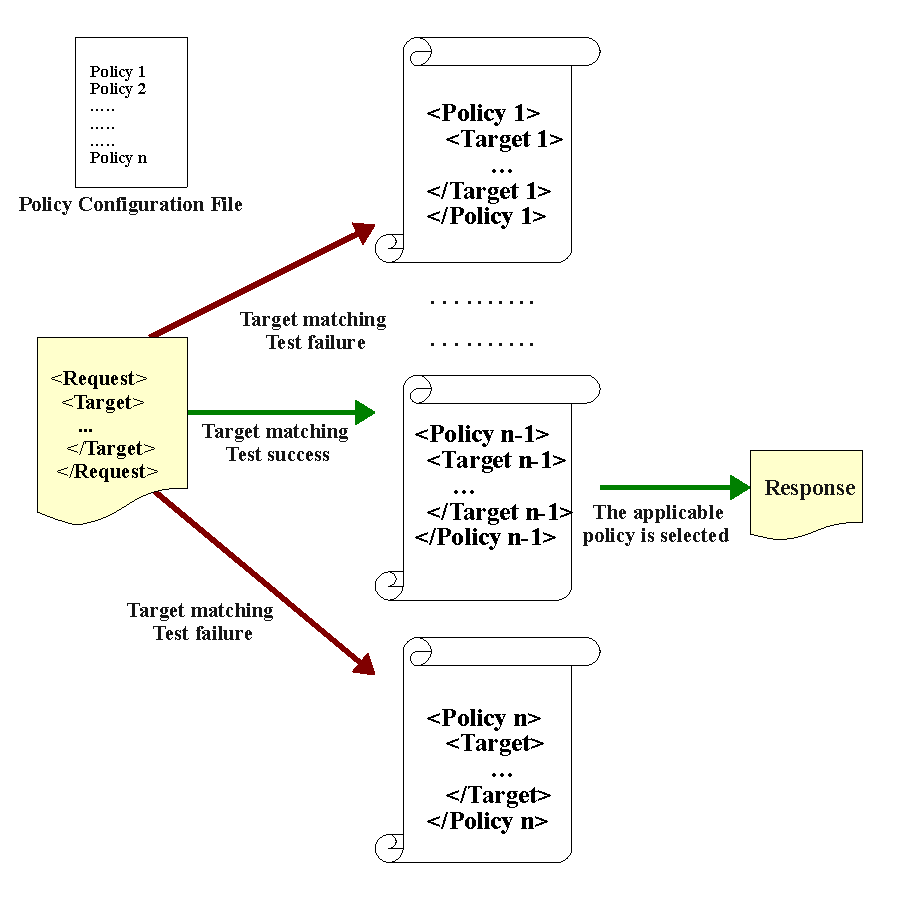
\includegraphics[width=3in, height=3in]{requestevaluation}
\caption{Applicable policy selection through target matching testing}
\label{requestevaluation}
\end{center}
\end{figure}



\subsection{Architecture Model Preservation: PEP-PDP Synergy}
We consider the different splitting criteria that we have identified in the previous section and we propose to select the splitting criterion that 
enables to preserve the synergy requirement in the access control architecture. This splitting criterion respects how PEPs are organized 
at the application level and how they are linked to their corresponding PDPs.

In the worst case, splitting the initial PDP into multi-PDPs may lead to a non-synergic system: a PEP may send its requests to several PDPs. 
The PDP, which receives a request is only known at runtime. Such a resulting architecture breaks the PEP-PDP synergy and the conceptual 
simplicity of the initial architecture model. 
A deep analysis of the PEPs at the application enables to observe the mapping between the PEPs and the PDP. At the application level, the PEP
is represented by a method call that triggers a decision making process by activating some specific rules in the PDP.
The code in Figure \ref{PEP deployment Example} is taken from \cite{legacy}, this code excerpt shows an example of a PEP represented by the method checkSecurity which calls the class 
SecurityPolicyService that initiates the PDP component.


An analysis of this code reflects that the PEP presented by the method ServiceUtils.checkSecurity will trigger exclusively all the rules 
that have the subject user (provided as input parameter in the PEP) and fixed Action (LibrarySecurityModel.BORROWBOOK\_METHOD) and Resource ( LibrarySecurityModel.BOOK\_VIEW).
Thus the splitting process that will preserve the mapping between the PEPs and the PDP will be $SC_{2}=<Resource,Action>$ in this case since the rules in the policy are triggered 
by Action, Resource. Depending on the organization of the PEPs in a given application, connecting the rules with their PEPs at the application level may require to identify
 all the enforcements points in the application, and to track the different method calls triggered from these specific enforcement calls to map them to the relevant access control rules.
Considering a strict mapping between a PEP and a sub-policy resulting from a splitting process enables to insure the synergy requirement in the access control architecture 
and preserves the simplicity of the initial architecture, by keeping a many-to-one association from PEPs to PDPs. A given request evaluation 
triggered by one PEP will always be handled by the same PDP. Operationally, the request evaluation process will involve 
one XACML policy file. In this case, the refactoring is valid, since its does not impact the conceptual architecture of the system.
Our empirical results, presented in section~\ref{sec:experiment}, have shown that adopting a policy refactoring based on system functions, as a refactoring strategy, enables to 
have the best splitting criterion in term of performance. 
In this work we consider 3 evaluation studies where the PEPs trigger (action, resource) in the policies, thus the splitting criteria $SC_{2}=<Resource,Action>$ is considered as 
the best splitting criteria that enables to preserve the synergy requirement in the architectural model. Inferring automatically the PEPs from the application enables to provide for a given 
application the best splitting criteria, this can be easily applied using the testing technique presented in \cite{legacy}.

As depicted in Figure \ref{overallprocess}, the refactoring process is automated and starts by specifying and creating the XACML file which 
will be split by our tool according to a specified SC that can be chosen by an access control stakeholder. Afterwards, the policies are included in the 
framework that supports our approach. For every change in the access control policy, the initial policy is updated and 
split again in order to be included again in the framework.
From a point of view of the system administration, maintaining and updating the access control policies is completely a standalone and simple
 process. The input is usually a centralized XACML policy. This input remains the same than before the access control performance issue is tackled.
Our process is transparent in the sense that it does not impact the existing functional aspects of the access control management system, 
for system administrators, who have to update the policy fequently and have to manage various dimensions of access control 
systems such the scalability and maintainability.
\begin{figure}[!h]
\begin{center}
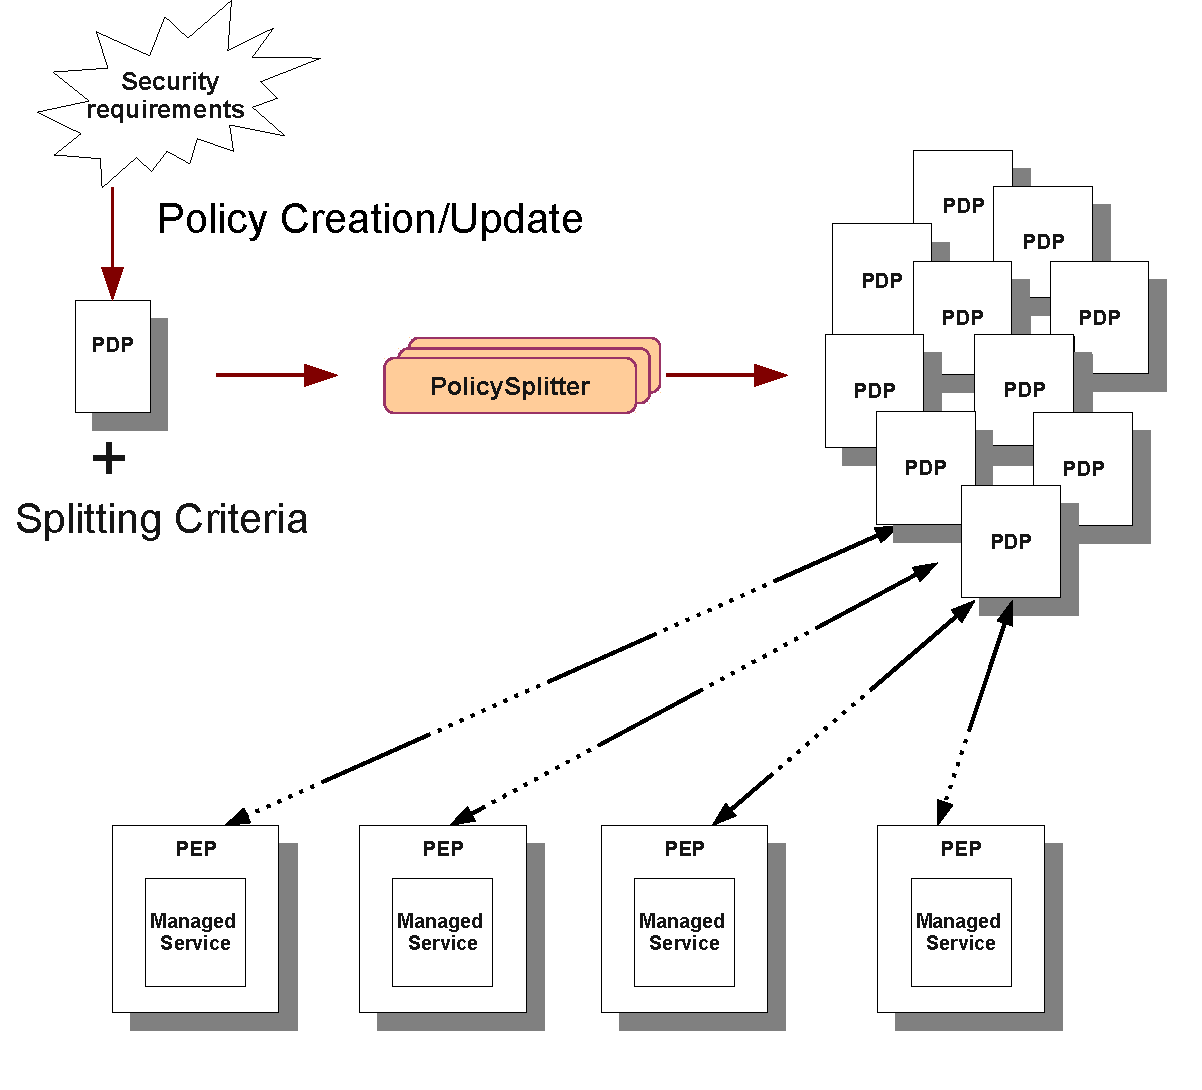
\includegraphics[width=8.5cm, height=8cm]{Overall-process}
\caption{Overview of the process of defining and deploying Access Control Policies}
\label{overallprocess}
\end{center}
\end{figure} 